Chapter~\ref{chapter:detection} and Chapter~\ref{chapter:fruit_counting} presented multiple techniques for fruit detection and counting. Combining per-frame detection and counting, we can obtain fruit counts for a single image. In natural settings though, fruit count from a single image is not reliable. Visibility of a particular fruit cluster varies drastically with the change in camera position (i.e. A cluster might be completely invisible/partially visible from a particular view and yet clearly visible from other views). To resolve these issues, majority of the yield mapping systems~\cite{bargoti_deep_2017,wang,stein_image_2016,gongal_apple_2016,das_devices_2015} including the methods developed in this dissertation capture a video of all the trees under consideration from a predefined trajectory and utilize information from all the views to obtain a robust estimate of the fruit count.

In this setting, each fruit may appear multiple times in different frames. Therefore, tracking becomes an essential task to avoid double counting of fruit. We need to track the fruit in the images captured from one side of a tree row as well as from the opposite side of owing to fruit visible from both sides. 

In this chapter, we present a method for tackling single-side tracking. Compared to existing tracking techniques, our method does not require specialized hardware~\cite{wang,gongal_apple_2016} and is capable of extracting fruit size along with the count. Essentially, our method recovers the underlying scene structure and camera motion. This is a very well studied problem in the field of computer vision known as Structure from Motion (SfM)~\cite{sinha2014multi}. In  a standard SfM pipeline (Fig.\ref{fig:sfmpipelines}(\subref{fig:standardsfm})) features such as SIFT~\cite{surffeature} or SURF~\cite{sift} are detected and matched across images. These matches are then used to estimate the geometry of the scene. Such methods fail in our application for two reasons:
\begin{description}
\item[Features] Often, point features such as SURF and SIFT are not detected on fruit. Even when found, in the presence of occlusions and specularities these features can generate zero or false matches. Remaining correct matches are too sparse to estimate diameters.
\item[Geometry] Baseline SfM methods fail to align dense fruit clusters across multiple frames resulting in the same fruit being registered multiple times (Fig.\ref{fig:pnpbase}).
\end{description}

To resolve these issues, in this chapter, we present a novel SfM pipeline where detected fruit contours are directly used for generating dense point matches. These matches are then used for estimating the motion of the camera and reconstructing the fruit in 3D. It should be noted that reconstruction from a single camera is bound to have global scale ambiguity (we can not know the scale without knowing the distance to the scene and vice versa). Our method fixes the reconstruction scale across the images and normalizes the sizes with respect to a reference fruit. This fruit can be identified and measured by the user to obtain diameter information in a given unit (e.g. centimeters).

\section{Assumptions on Camera Calibration}
In developing our algorithms, we made a few assumptions about the setup. First, we assume that the camera is intrinsically calibrated. While auto-calibration techniques can be incorporated into
the pipeline, we have not investigated this extension. It should also be noted that newer platforms such as Google Tango Tablet are making calibration parameters available to developers. As a result of the calibration assumption, we require the camera to have a fixed focus. A camera whose focus changes dynamically (i.e auto-focus) is not compatible with our system.  Most of the cameras in smartphones and tablets have fixed focal length and can be used for data collection (the auto-focus functionality in these cameras does not change the true focal length and camera center).  Cameras with variable focal length can be used after fixing the zoom and focus.  We have used the calibration toolbox and the standard chessboard pattern to calibrate the cameras~\cite{camcalib}.


\section{Computation of Dense Feature Matches} \label{sec:affinetrans}

In an orchard setting, usually, only the frontal views of the fruit clusters are available. Even from a few meters for ellipsoidal fruit (e.g apples, oranges, strawberries, lemons, etc.), the depth change in the visible portion is negligible and the fruit geometry can be approximated by a circle lying on a plane. This allows us to assume that matching fruit across individual fruit clusters in consecutive images are related by an affine transformation. We apply a nonlinear optimization method based on Gauss-Newton gradient descent as described in~\cite{Kannade} to recover these affine transformations. In this section, we present the equations for fruit contour alignment.

Given two fruit contours, the  affine transformation relating them is parameterized in the following way,


$$
A(p)=
  \begin{bmatrix}
    1+p_1 & p_3 & p_5 \\
    p_2 & 1+p_4 & p_6
  \end{bmatrix}
 $$


We seek the transformation $A$ which minimizes
\begin{equation}
\sum_{\bar{x}} [ I_2(\bar{x}) - I_1(A(\bar{x})) ]^2
\end{equation}
 where, $I_1$ and $I_2$ are the corresponding fruit clusters and $\bar{x}$ is the homogeneous vector representation of image coordinates $[u,v,1]^T$. Here, $I_2$ can be thought of as a template and  $I_1$ as an image that is to be aligned to the template after going through the affine transformation $A$. Note that we seek to compute a separate affine transformation for each fruit cluster.
 The inverse compositional algorithm~\cite{Kannade} seeks to minimize, 
 
 \begin{equation}
 \argmin_{\Delta p} \sum_x \left[  I_2(A(\Delta p) \bar{x}) - I_1(A(p)\bar{x})\right]^2
 \label{eq:afwarp}
 \end{equation}

here $\Delta p$ is the incremental transformation to be applied to the existing affine warp $A(p)$. This warp is applied in the following way:

$$A(p) \leftarrow A(p) * A(\Delta p)^{-1}$$
As evident from the name, the incremental warp has to be inversed before composing with current warp. Performing a first order Taylor expansion of equation~\eqref{eq:afwarp} we get,

$$ \sum_{\bar{x}}\left[I_2(A(0)\bar{x}) + \Delta I_2 \frac{\delta A}{\delta p} - I_1(A(p)\bar{x})\right]^2$$

If we assume that the initial warp $A(0)$ is identity, the incremental warp $\Delta p$ can be computed as a least square solution to the above equation, 

$$\Delta p = H^{-1}\sum_{\bar{x}}\left[\Delta I_2 \frac{\delta A}{\delta p}\right]^T \left[I_1(A(p)\bar{x}) - I_2(\bar{x})\right]$$
where the Hessian is
$$H = \sum_{\bar{x}}\left[\Delta T \frac{\delta A}{\delta p}\right]^T \left[\Delta T \frac{\delta A}{\delta p}\right]$$

The details of the algorithm can be found in the inverse compositional algorithm section in ~\cite{Kannade}. In step (2) of the inverse compositional algorithm~\cite{Kannade} the error image is obtained as plain subtraction (i.e $I_1(A(p)*\bar{x}) - I_2(\bar{x})$). This step is changed in our implementation to penalize the warps that map the image points outside the template. We impose a heavy cost whenever the warped points are outside the template. 

Following the computation of dense matches, we can formulate an affine hierarchy between the matching contours across images and identify them uniquely. Fig.\ref{fig:totalaffine}(\subref{fig:affinemap}) shows such an example. Affine transformation $A_{1,2}^1$ maps contour $C_1$ in image $I_1$ to $I_2$ and affine transformation $A_{2,3}^1$ maps contour $C_1$ from image $I_2$ to $I_3$. Therefore the affine transformation relating contour $C_1$ from frame $I_1$ to frame $I_3$ is $A_{1,2}^1 * A_{2,3}^1$. We emphasize the novelty of our approach that different contours are related by different affine transformations (For contour $C_2$ we have a different affine hierarchy). The obtained dense matches and segmented images are next fed into our novel SfM pipeline, which is discussed in the next section.




\begin{figure*}[!htbp]
        \centering

        \begin{subfigure}[t]{.8\textwidth}
                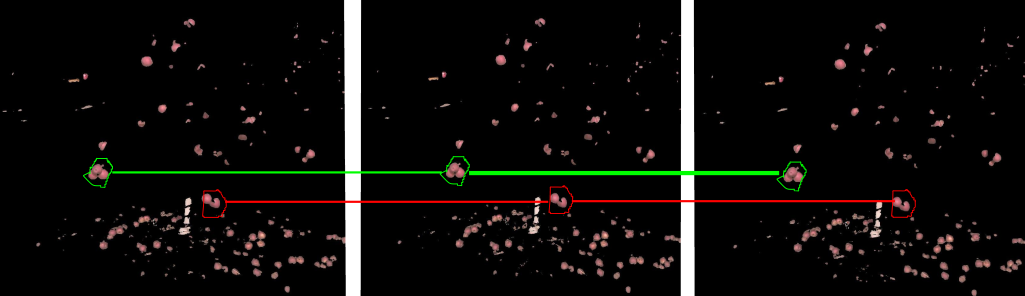
\includegraphics[width=\textwidth]{figures/isfm/contourmaps.png}
                \caption{Matching between contours.}
                \label{fig:fcond}
        \end{subfigure}        
        
        \begin{subfigure}[t]{0.3\textwidth}
            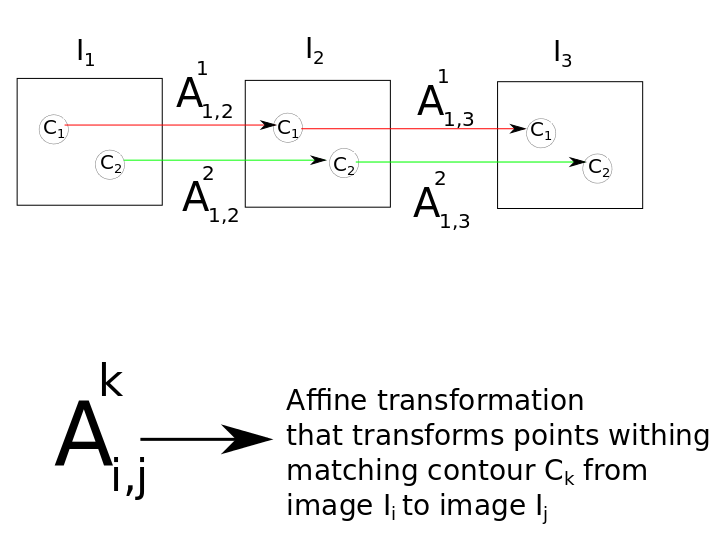
\includegraphics[width=\textwidth]{figures/isfm/affinemap.png}           
         \caption{Affine Map}
         \label{fig:affinemap}
       \end{subfigure} \quad \begin{subfigure}[t]{0.5\textwidth}
                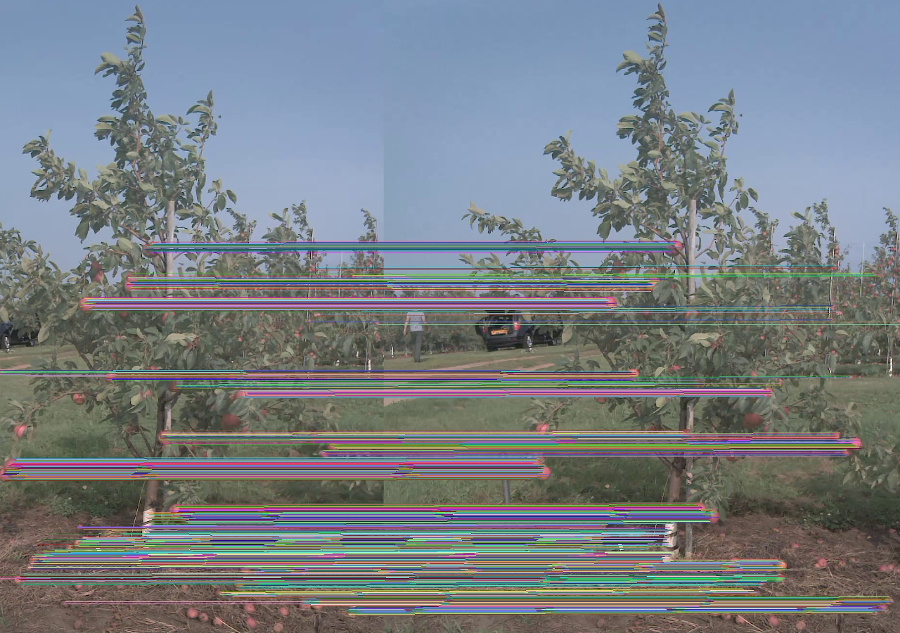
\includegraphics[width=\textwidth]{figures/isfm/MatchingBetweenImages1.jpg}
                \caption{Dense matching between images \label{fig:densematch}}
                \label{fig:matching}
        \end{subfigure}
       
        
        
        
        \caption[Using fruit as features for dense correspondences]{Computation of dense matching through affine transformation. For clarity only 10\% of the matches are shown.}
        \label{fig:totalaffine}
\end{figure*}

\section{The Structure from motion pipeline}\label{sfm}

Most of the standard feature-based sequential SfM pipelines operate by selecting a pair of good initial frames for reconstruction (Fig.\ref{fig:sfmpipelines}(\subref{fig:standardsfm}))~\cite{scaramuzza2011visual}. After reconstructing the initial structure, each additional frame is matched to the frames already used in the reconstruction. The reprojection error between reconstructed world points and matching points in the new frame is minimized to recover the camera pose and introduce new points to the structure ~\cite{pnp}. Another standard approach is to do two/three-view reconstruction and then merging them using the constraints enforced by the common view~\cite{sinha2014multi}. Both these standard approaches work well for sparse reconstructions in the presence of a large number of non-planar features. In contrast, we have dense features from fruit but many of them are planar. These standard approaches fail to align the reconstructed fruit in different frames even with the aid of costly non-linear bundle adjustment (Fig.~\ref{fig:pnpbase}).


\begin{figure}[!htbp]
\centering
\begin{subfigure}[t]{0.8\textwidth}
    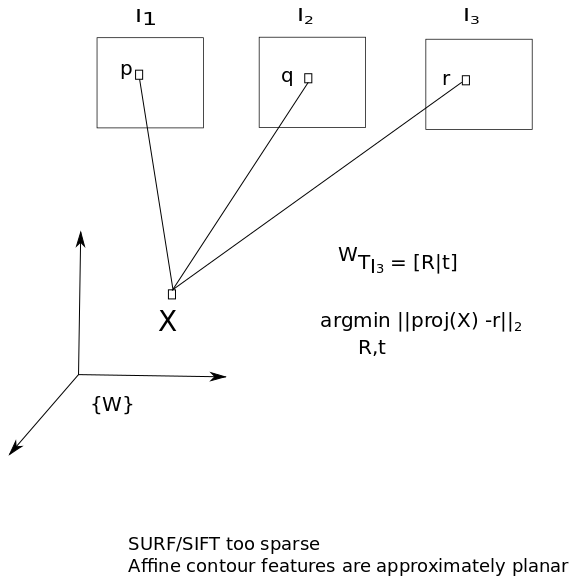
\includegraphics[width=0.8\textwidth]{figures/isfm/standardSFM.png}
\caption{A standard PnP based SfM pipeline}
\label{fig:standardsfm}
\end{subfigure}\quad \begin{subfigure}[t]{0.8\textwidth}
    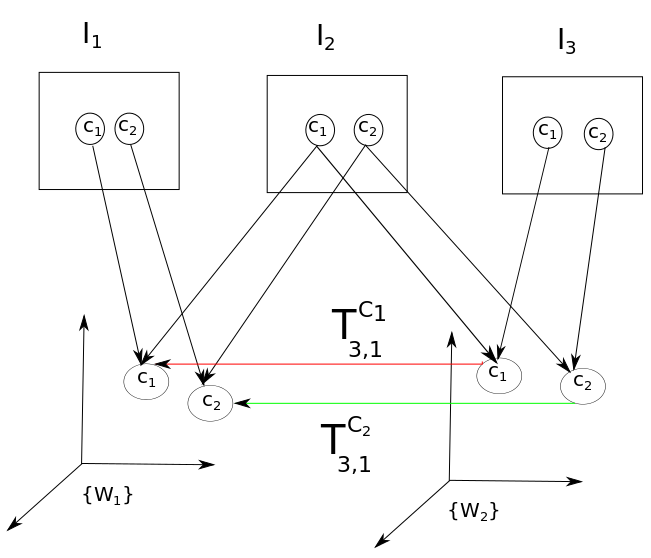
\includegraphics[width=0.8\textwidth]{figures/isfm/OurSFM.png}
        \caption{Our piecewise incremental SfM pipeline}
        \label{fig:oursfm}
        \end{subfigure}
        
        
        \caption[Comparison of a common structure from motion (SfM) pipeline and our pipeline.]{ Comparison of a common SfM pipeline and our pipeline. On Fig(\subref{fig:standardsfm}) we show a common structure from motion pipeline. It operates by constructing an initial structure. Then it incrementally augments the structure by adding new points from subsequent frames by solving the Perspective n Point (PnP) 2D to 3D correspondence problem. In the figure, matching points $p$,$q$ and their reconstruction $X$ is shown. The next camera pose is determined by minimizing the reprojection of the world point $X$ to matching image point $r$. On Fig(\subref{fig:oursfm}) we show Our SFM pipeline. Instead of aligning entire frames, we align the fruit clusters individually. The average scale factor of these individual alignments are used to align non-matching clusters.}
\label{fig:sfmpipelines}
\end{figure}


 \begin{figure}[!htbp]
        \centering
\begin{subfigure}[t]{.23\textwidth}
                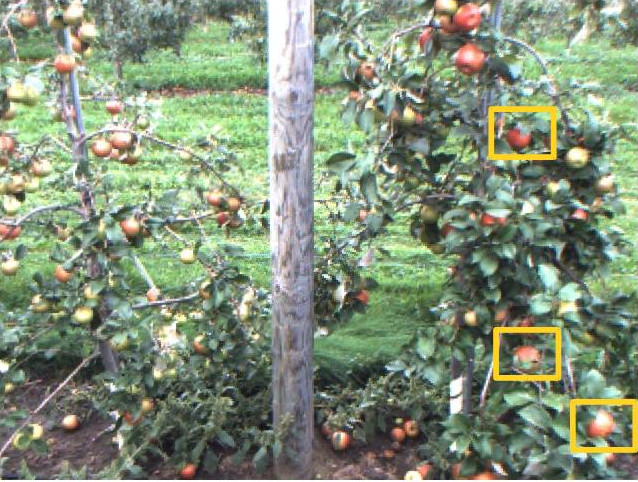
\includegraphics[width=\textwidth]{figures/isfm/original.jpg}
                \caption{Reference view}
                \label{fig:orig}
        \end{subfigure} \begin{subfigure}[t]{.23\textwidth}
                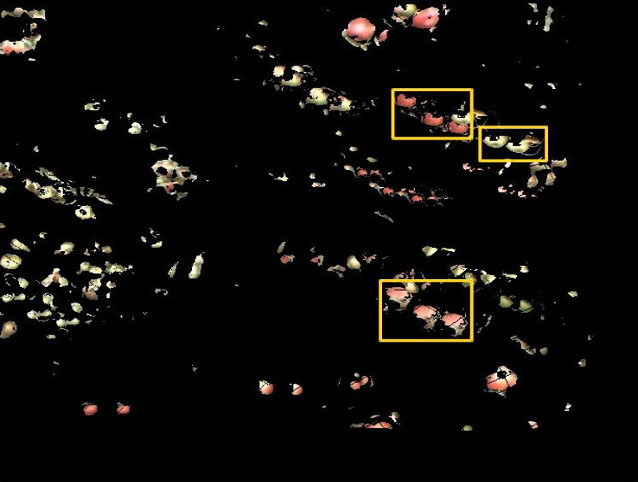
\includegraphics[width=\textwidth]{figures/isfm/isfmreproj1.jpg}
                \caption{Baseline incremental SfM}
                \label{fig:isfmbase}
        \end{subfigure} \begin{subfigure}[t]{.23\textwidth}
                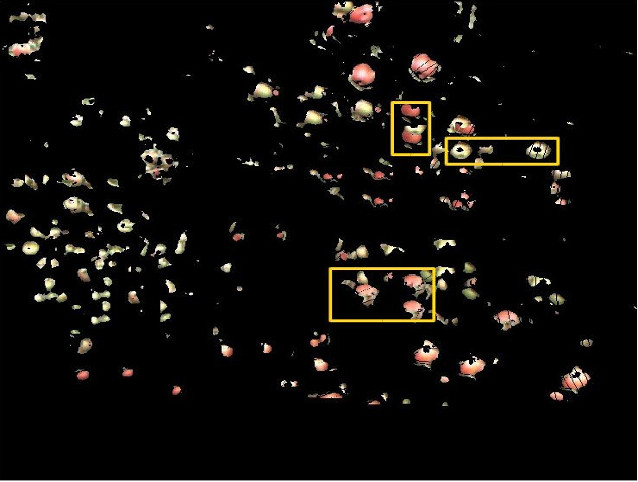
\includegraphics[width=\textwidth]{figures/isfm/pnpreproj1.jpg}
                \caption{PnP based SfM}
                \label{fig:pnpsfmbase}
        \end{subfigure} \begin{subfigure}[t]{.23\textwidth}
                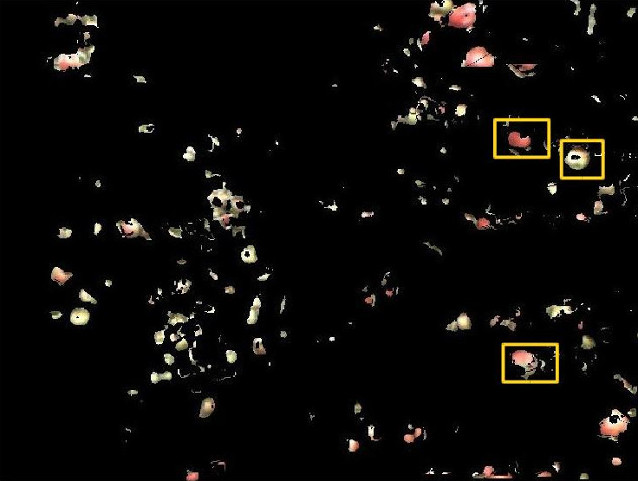
\includegraphics[width=\textwidth]{figures/isfm/ourreproj.jpg}
                \caption{Our pipeline}
                \label{fig:reconnooverlap}
        \end{subfigure}
        
        \caption[Failure of baseline incremental structure from motion (SfM) and PnP~\cite{pnp} based methods to align dense fruit clusters.]{Failure of baseline incremental SfM and PnP~\cite{pnp} based methods to align dense fruit clusters. Fig(\subref{fig:orig}) shows the reference image to which we project all the 3D points from our reconstruction. Fig(\subref{fig:isfmbase}) shows a reprojected image frame from the baseline incremental SfM reconstruction and Fig(\subref{fig:pnpsfmbase}) shows a reprojected image frame from a PnP based reconstruction. Both images contain the same fruit multiple times (some of them are shown in rectangular boxes) which shows the inability of these methods to register the clusters successfully. In Fig(\subref{fig:reconnooverlap}) we show the same image in Fig. ~\ref{fig:pnpbase} obtained from our pipeline. It solves the problem of multiple registrations of the same fruit observed while applying the baseline methods.}
 \label{fig:pnpbase}
\end{figure}

To resolve this problem, we propose a novel piecewise incremental structure from motion pipeline (Fig.\ref{fig:sfmpipelines}(\subref{fig:oursfm})). Similar to most incremental methods, our pipeline operates by pairwise reconstruction and merging the reconstructed point-clouds. As the cameras are calibrated, reconstructed points in different reference frames differ from each other by a similarity transformation. Our merging procedure utilizes the obtained affine relationship in the previous step to merge the reconstructions. Instead of solving for the transformation between two reference frames, we solve for the transformation between the matching fruit clusters and align them individually.


Our novel pipeline for dense structure from motion has three steps:
\begin{enumerate}
\item Keyframe selection and pairwise reconstruction
\item Alignment of reconstructed point-clouds using cluster-wide  transformation 
\item Computation of  overall camera motion and optional bundle adjustment
\end{enumerate}





%\begin{figure}[htb]
%\centering
%\includegraphics[width=0.8\textwidth]{./figs/visualsfmsparse}
%\caption{Visual SFM sparse reconstruction from three hundred frames. Dense reconstruction with PMVS does not get any point. The two images in Fig.\ref{fig:densematch} were part of the input}
%\label{fig:visualsfmsparse}
%\end{figure}

We describe each of these steps in details in the following:

\subsection{Keyframe Selection and Pairwise Reconstruction}\label{subsec:pairwiserecons}

To do precise reconstruction from an image sequence we need to ensure that frames within a pair satisfy the epipolar constraints, and have sufficient parallax between each other. Given the image sequence $I_1,I_2,...,I_n$ we choose an arbitrary frame $I_m$ where $m\in \{1,2,...n\}$, as the first frame. Then we find another frame $I_{m+i}$ which is consistent with frame $m$ in terms of epipolar constraints. We perform pairwise reconstruction in the following way:

\begin{enumerate}


\item As the correspondence problem has already been solved in a previous step, we have dense feature matches between the images. To ensure enough parallax we compute both essential matrix $E$~\cite{nister} and homography between the images and then check whether they satisfy the Geometric Robust Information Criterion (GRIC) defined by Torr~\cite{torr1997assessment}. This criterion makes sure that the essential matrix is modeling the relationship between the frames better than homography. If the frames do not satisfy GRIC, we skip the current frame and move to the next one.

\item We decompose $E$ to find the $R$ and $t$ between the cameras as described in section 9.6.2 of ~\cite{hartley2003multiple}.
\item While decomposing $E$, if we find that, determinant($E$) is not
  close to zero (we use determinant($E$)$ < 1e-10$), or the two singular
  values (we use singular value ratio $<=.9$) of $E$ are not identical
  we reject the essential matrix and go to step 6.
\item The decomposition of $E$ yields four combinations of $R$ and $t$. We triangulate using each of these combinations and check for the cheriality condition (we checked whether $99\%$ of the reconstructed points are in front of the camera). If we find a valid triangulation with low average reprojection error (the threshold we use is $1.00$ pixels), we reconstruct using the obtained projection matrices. 

\item We impose one additional constraint on the triangulation angle to ensure the robustness of the reconstructed structure. Triangulated points for which the triangulation angle is within five to sixty degrees are kept and the rest are discarded. This is done to protect against parallel and vertical triangulation rays that lead to poor structure~\cite{parsonage2011efficient}.

\item If we do not find a valid triangulation or we reject the essential matrix because of not satisfying the criteria in step 4, we discard the current frame and move to the next one.

\end{enumerate}

Following these steps we reconstruct using the matches from the image pair, $< I_m, I_{m+i}>$.  We assume our world/reference frame is the first camera frame. Next, we look for a subsequent frame that is consistent with frame $I_{m+i}$ using the same procedure described above and reconstruct from the found pair. If none of the subsequent image frames are consistent with frame $I_{m+i}$, we discard one of the initial frames (e.g discard $I_{m+i}$ and find a new suitable frame for pairwise reconstruction with frame $I_m$ and continue in this way). As mentioned previously, the first camera frame used for reconstructing the initial pair acts as the frame of reference. Proceeding this way, we have multiple pairwise reconstructions, none of which are aligned. In the following section, we describe how to align these reconstructed point-clouds.



% Figure ~\ref{epipolar} shows the epipolar lines in two images used for reconstruction.
%\begin{figure}[htb]
%\centering
%\includegraphics[width=0.8\textwidth]{./figs/EpipolarLines}
%\caption{Epipolar Lines in two images used for reconstruction. The parallel lines suggest the corresponding camera motion is perpendicular to the image plane}
%\label{fig:epipolar}
%\end{figure}


\subsection{Alignment of reconstructed point-clouds using cluster-wise  transformation}\label{subsec:alignment}

The alignment proceeds by calculating the transformation $T^{C_m}_{i,j}$ between matching reconstructed fruit cluster $C_m$ between reference frame $i$ and $j$. Let $^i{C_m}$ denote the reconstructed cluster in reference frame $i$ and $^j{C_m}$ denote the reconstructed cluster in reference frame $j$. Here, the reference frames also denote corresponding camera reference frames. The reconstruction in reference frame $i$ is obtained from image pairs $<I_i, I_j>$ and reconstruction in reference frame $j$  is obtained from pair $<I_j,I_k>$. So, 
\begin{equation}
^i{C_m} =\  ^iR_j ^j{C_m} + \lambda_i ^iT_{j_{org}}
\label{eq:fri}
\end{equation}


where $^i R_j,^iT_{j_{org}}$ is the rotation and translation mapping reference frame $j$ to $i$, $\lambda_i$ is the lost scale factor while extraction of translation from essential matrix. If $i$ is our base reference frame (i.e all other reconstructions will be mapped to this frame), without loss of generality we can set $\lambda_i = 1$. All other frames will be reconstructed up to the scale of the initial reconstruction in base frame $i$. Moving onto the next reconstruction of cluster $C_m$ in reference frame $j$,
\begin{equation}
^j{C_m} =\ ^jR_k ^k{C_m} + \lambda_j ^jT_{k_{org}}
\label{eq:frj}
\end{equation}


Replacing the value of $^j{C_m}$ in equation~\eqref{eq:fri} from equation~\eqref{eq:frj} we obtain:
\begin{equation}
^i{C_m} =\ ^i R_j(^jR_k ^k{C_m} + \lambda_j ^jT_{k_{org}}) + \lambda_i ^iT_{j_{org}}
\label{eq:frfinal}
\end{equation}

Using the correspondences from the cluster $C_m$ in equation~\eqref{eq:frfinal} we can solve for the scale factor $\lambda_j$. Then the points in the reconstruction of $^j C_m$ in reference frame $j$ which do not correspond to any points in $^i C_m$ can be aligned to base frame $i$ using the right side of equation~\eqref{eq:frfinal}. An illustration of this procedure can be found in Fig.\ref{fig:sfmpipelines}(\subref{fig:oursfm}). As equation~\eqref{eq:frfinal} uses only correspondences within a cluster $C_m$ and therefore the obtained scale is local with respect to the reconstructed points in $^i C_m$. If we average all of these local scales, we will obtain a scale consistent across the entire point-cloud.  This scale is used to align the point-clouds of clusters that do not have corresponding matching clusters in the previous reconstruction.
 \begin{figure}[!h]
       \centering
       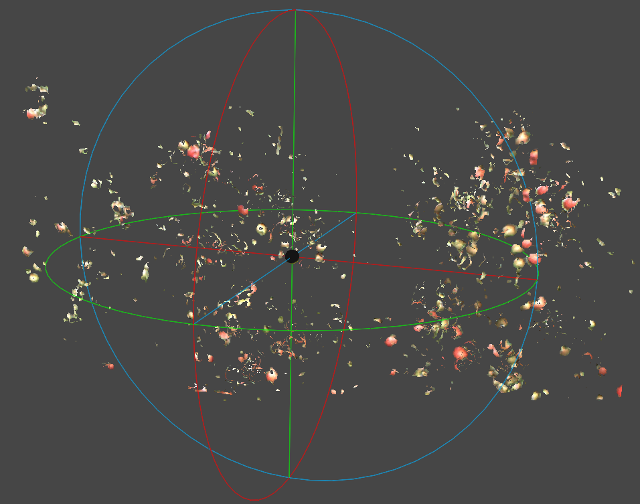
\includegraphics[width=.7\textwidth]{figures/isfm/3dcircle1.png}
        \caption[Dense reconstruction from our pipeline.]{Dense reconstruction from our pipeline. We show a sample reconstruction of three trees from our novel SfM pipeline. The circles are shown for illustration purposes.}
\label{fig:recon}
\end{figure}



\subsection{Computation of  overall camera motion and optional bundle adjustment}
\label{subsec:camera motion}
The retained overall scale in the previous step defines the additional camera pose up to a consistent scale. The pose for camera k is,  $^jT_k = \left[^jR_k|\lambda_G ^j T_{k_{org}}\right]$, where $\lambda_G$ denote the overall scale. In conventional incremental SfM, this step is followed by a bundle adjustment~\cite{bunad}. The robustness of the piecewise alignment enables us to skip this step. Fig.\ref{fig:reprojmultiple} shows, even without bundle adjustment the reprojection error is much lower than the baseline incremental and PnP based methods. Nevertheless, we perform bundle adjustment as the final step of the reconstruction procedure. It helps to remove small drifts in the camera motion resulting in a robust estimation of both structure and motion (Fig.~\ref{fig:cammotion}).


\section{Application for Diameter Estimation}\label{sec:estimation}
As fruit clusters are tricky to separate into individual fruit, we select only single fruit for diameter estimation. This is ensured by the counting method described in chapter~\ref{chapter:fruit_counting}. To compute the diameters, we use the diameter estimation method in \cite{techreport }. This method essentially finds the pixel diameter and the average depth of the pixels within the fruit. Then it projects the pixel diameter to average depth to find the metric diameter. As our reconstruction is only up to a scale, the obtained diameter is also defined up to a scale. We fix the diameter of a random fruit in a metric unit to obtain the required scale factor. This scale factor is used to convert our obtained up to scale diameters to metric units. The metric diameter of the random fruit is a user input in our estimation system. In the section, ~\ref{subsec:evalest} we evaluate our counting and diameter estimation procedures rigorously.


\section{Experimental Results on Apple Orchard Data }\label{sec:experiments}
In this chapter, we presented an SfM pipeline that can obtain a dense reconstruction of orchard rows and estimate fruit counts and diameters. To validate this approach we collected two datasets (using both stereo and monocular cameras) from the apple orchards at the University of Minnesota Horticulture Research Center: 
\begin{itemize}
\item Dataset1 primarily contains red Apples. The total number of images is $965$. Sample images from the dataset are shown in Fig.~\ref{fig:datasets_isfm}. These images cover a full row of an orchard.
\item Dataset2 contains a mixture of red and green apples. The total number of images is $464$. Sample images from the dataset are shown in Fig.~\ref{fig:datasets_isfm}. This dataset covers one block containing six trees.
\end{itemize}


\begin{figure*}[!h]
        \centering

        \begin{subfigure}[t]{.35\textwidth}
                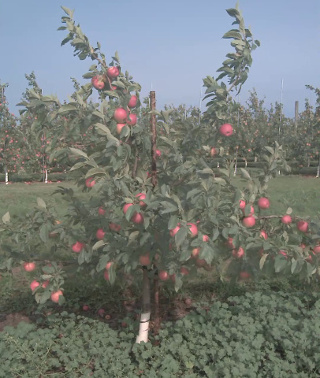
\includegraphics[width=\textwidth]{figures/isfm/dataset11.jpg}
                %\caption{Sample image from the first dataset}
                \label{fig:dataset1}
        \end{subfigure}\quad \begin{subfigure}[t]{.55\textwidth}
                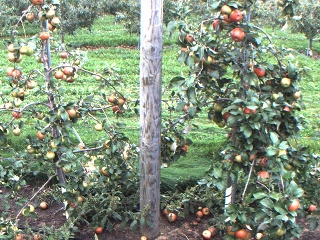
\includegraphics[width=\textwidth]{figures/isfm/dataset21.jpg}
                %\caption{Sample image from the second dataset}
                \label{fig:dataset2}
        \end{subfigure}
       
        
        
        
        \caption[Sample images from used datasets.]{Sample images from used datasets. The figure on left shows a sample image from Dataset1 primarily containing red apples. The figure on right shows a sample image from Dataset2 containing a mixture of red and green apples.}\label{fig:datasets_isfm}
\end{figure*}





We tested both our SfM pipeline and yield estimation capabilities using these two data sets.
\subsection{Evaluation of the novel SfM pipeline}
\label{subsec:evasfm}
Our SfM pipeline uses a piecewise incremental process to recover camera motion and scene structure. The figures (Fig. \ref{fig:cammotion}, \ref{fig:reprojmultiple}) are produced from over 200 frames in Dataset2. The figures show only the keyframes selected by our SfM pipeline. Even without the aid of bundle adjustment the reprojection error (Fig.~\ref{fig:reprojmultiple}) is very low. However, the camera motion without bundle adjustments has small drifts as shown in Fig. ~\ref{fig:cammotion}. The bundle adjustment procedure eliminates these small drifts and corrects the camera motion and scene structure.

\begin{figure}[!h]
        \centering

        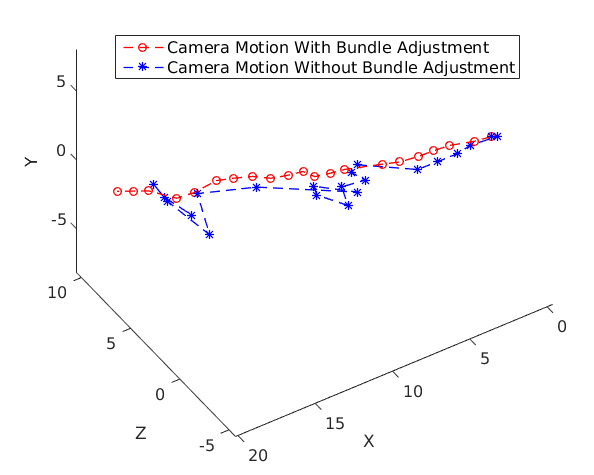
\includegraphics[width=\textwidth]{figures/isfm/CameraMotion.png}
       
 \caption{The computed camera motion with and without bundle adjustment. Bundle adjustment removes the drifts in camera motion.}\label{fig:cammotion}

\end{figure}
        
        

%\begin{figure}[htb]
%\centering
%\includegraphics[width=\textwidth]{./figs/reprojPiecewise1}
%\caption{Average pixel reprojection error with and without the application of bundle adjustment. Although bundle adjustment decreases the pixel reprojection error, with the robust piecewise scaling the reprojection error is already very low compared to the baseline methods (Fig.~\ref{fig:reprojmultiple})
%\label{fig:reproj}}
%\end{figure}


We compare our method with the two popular baseline methods: incremental SfM and PnP based SfM. Both methods are implemented with full bundle adjustment after the addition of each new frame. The results show that even without bundle adjustment our piecewise incremental method has lower reprojection error than the baseline methods (Fig.~\ref{fig:reprojmultiple}).


\begin{figure}[!h]
\centering
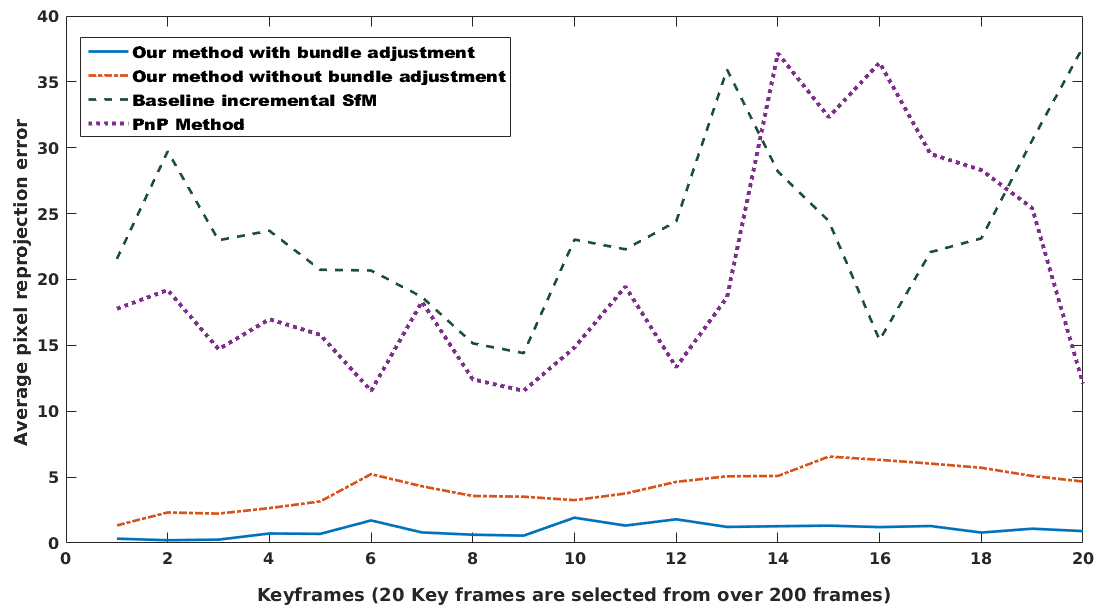
\includegraphics[width=\textwidth]{figures/isfm/reprojmultiple2.png}
\caption[Reprojection error for our method with and without bundle adjustment, baseline incremental structure from motion (SfM) and PnP based SfM.]{Reprojection error comparison. Our piecewise incremental method performs better than both baseline methods even without bundle adjustment. Bundle adjustment though reduces the reprojection error further and helps to correct the small drifts and smooth camera motion as shown in Fig.~\ref{fig:cammotion}.
\label{fig:reprojmultiple}}
\end{figure}


\subsection{Field Results for Apple Diameter Estimation}
\label{subsec:evalest}

For evaluating diameter estimation using monocular cameras, we use stereo data as ground truth. The diameters from our SfM reconstruction is only up to a scale. To fix the scale, we randomly choose an apple and find the metric value of its diameter. The ratio of the obtained diameter from our pipeline and this metric value provides us with the scale factor needed to scale our diameter data. Fig. ~\ref{fig:diamplots} shows the histogram of obtained diameters from the stereo and single camera. We compared the diameters of a hundred single apples from the Datasets. The results show that the mean difference between monocular and stereo diameter is $+.90$ centimeters(cm) and the standard deviation is $\pm 2.9$ cm. To find the dissimilarity between the two distributions more rigorously, we used earth mover's distance~\cite{rubner2000earth}. The found dissimilarity between the two distribution is $.65$. In other words, to morph one distribution into another, the average distance per weight in the horizontal axis is less than one.





\begin{figure}[!h]
\centering
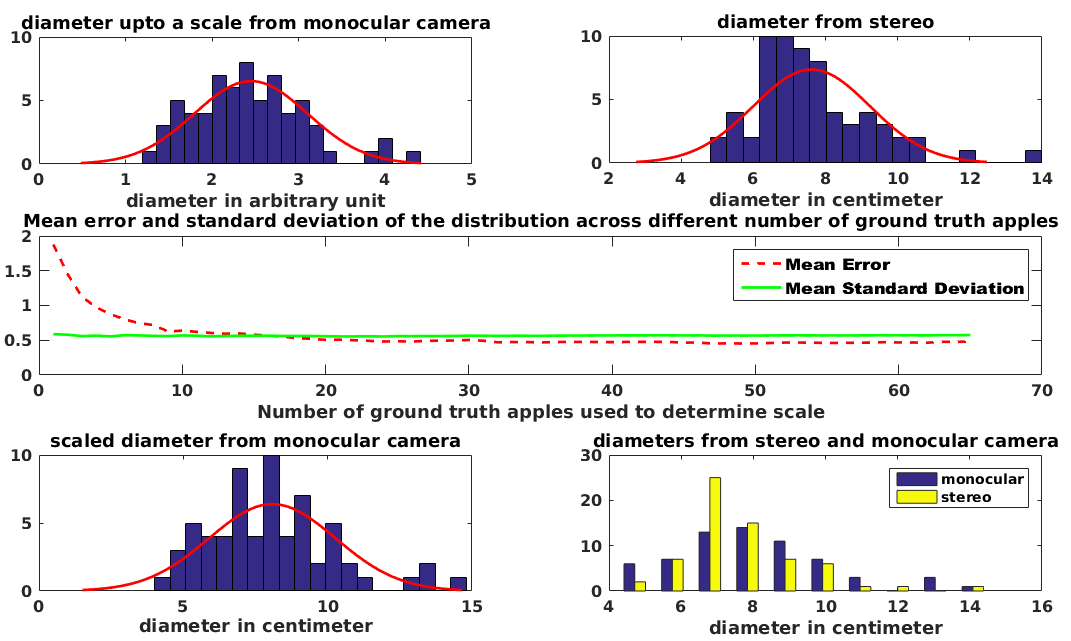
\includegraphics[width=\textwidth]{figures/isfm/diameterfull1.png}
\caption[Comparison of diameter estimation from our method with a single camera with stereo.]{Comparison of diameter estimation from Monocular Camera (top-left) with Stereo (top-right). 
Middle row: The scale can be estimated by measuring apples as ground truth. The error as a function number of apples used to estimate 
the scale. With four or more measurements, the error drops below one centimeter. Bottom row:
The scaled diameter estimation from our method (left) and  a side by side comparison of obtained histograms (right).}
\label{fig:diamplots}
\end{figure}


Using only one apple to scale up the scene can be susceptible to noise. To get accurate estimates we may need to choose multiple apples, find their actual diameter and find the average scale factor. Fig.\ref{fig:diamplots} shows how the error in the monocular estimate decreases with an increasing number of apples used for estimating scale. The results indicate that if we use more than four ground truth apples, the error drops below one cm.

\section{Conclusion}\label{sec:isfm_conc}

This chapter presented a method that can recover the underlying scene geometry and camera motion using the detected fruit themselves as features. Coupling this technique with existing dense multi-view stereo reconstruction algorithms~\cite{goesele2007multi} we can fully reconstruct the scene geometry from captured single side footage. The resulting 3D reconstructions are used to track the fruit and estimate fruit diameters up to scale. However, the obtained geometric representation is from a single side only. In the next chapter, we present a method capable of aligning independent reconstructions from both sides utilizing semantic features.